% section 3

\section{環境識別子とその精密化}

\subsection{環境識別子による変数のスコープ表現}
\kam{ここに須藤研究と大石研究の図をいれる(大石研究の図は、次の章に移動
  する予定だが、とりあえず、ここにいれておいてください)}

環境識別子 Environment Classifier による型による変数のスコープのアイデア\cite{Taha:2003:EC:604131.604134,Sudo2014}を拡張することによって,shift0/reset0の型安全性を保証する.
今まではプログラムがネストしていけば,その分だけ使える自由変数が増えていったのだが, shift0/reset0 が導入されたことにより,計算の順序が変わり,単純にネストした分だけ使える自由変数が増えていくという訳にはいかない.
そこで,環境識別子の結合を意味する $\cup$ を導入することにより上記の問題を解決することにした.


コードレベルの変数スコープと,型によるスコープの表現をあらわしたのが,以下の図である.
\begin{center}
  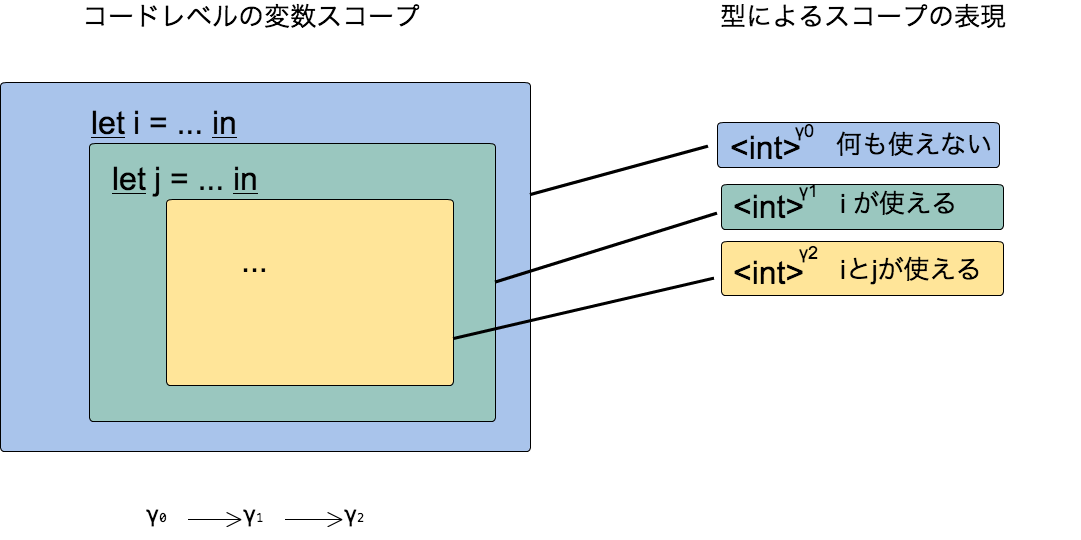
\includegraphics[clip,height=4cm]{./img/ec_let.png}
\end{center}

環境識別子とは,ある項のスコープの範囲において使える自由変数の集合である.
プログラムのネストが深くなると,使える自由変数が増えていくことが上図で分かるだろう.

\begin{center}
  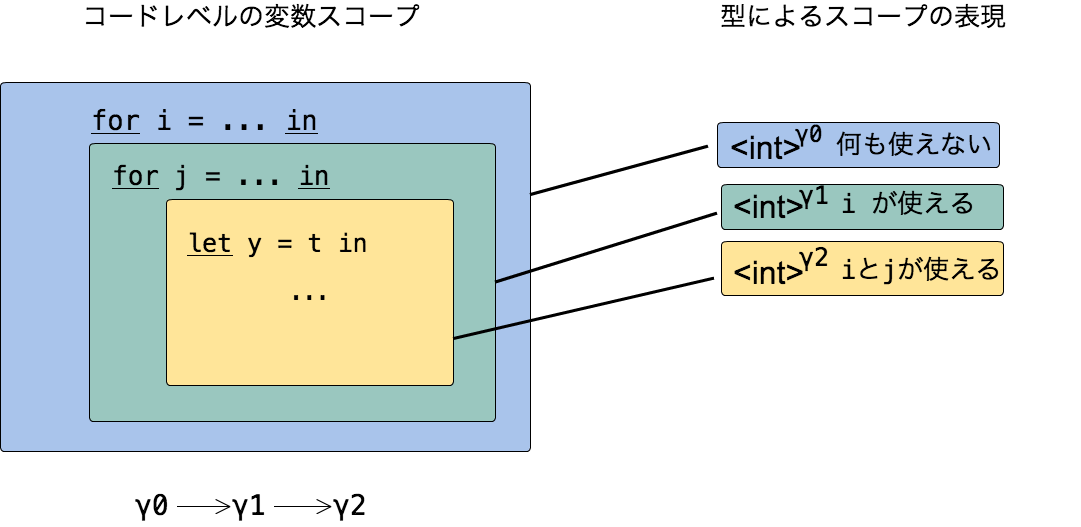
\includegraphics[clip,height=4cm]{./img/ec_for.png}
\end{center}

$\gamma$は変数のスコープを表し,そのスコープ内で使える自由変数の集合と思ってもらえば良い.
$\gamma$には,包含関係があり,それを $\gamma_1 \ord \gamma_0$ というような順序で表す.
直感的には$\gamma_0$より$\gamma_1$のほうが使える自由変数が多いという意味である.

このように EC を型に付加することで,その型がどのスコープに存在するかどうかが分かる.
つまり,型同士の相対的な位置を型レベルで判断できるようになる.

% \begin{tikzpicture}
%   \node (s) {$\gamma_0$};
%   \node[above right=of s] (a) {$\gamma_1$};
%   \node[below right=of s] (b) {$\gamma_2$};
%   \node[below right=of a] (t) {$\gamma_3 = \gamma_1 \cup \gamma_2$};

%   \foreach \u / \v in {s/a,s/b,b/t,a/t}
%   \draw[->] (\u) -- (\v);
% \end{tikzpicture}

\subsection{環境識別子の精密化}

\begin{center}
  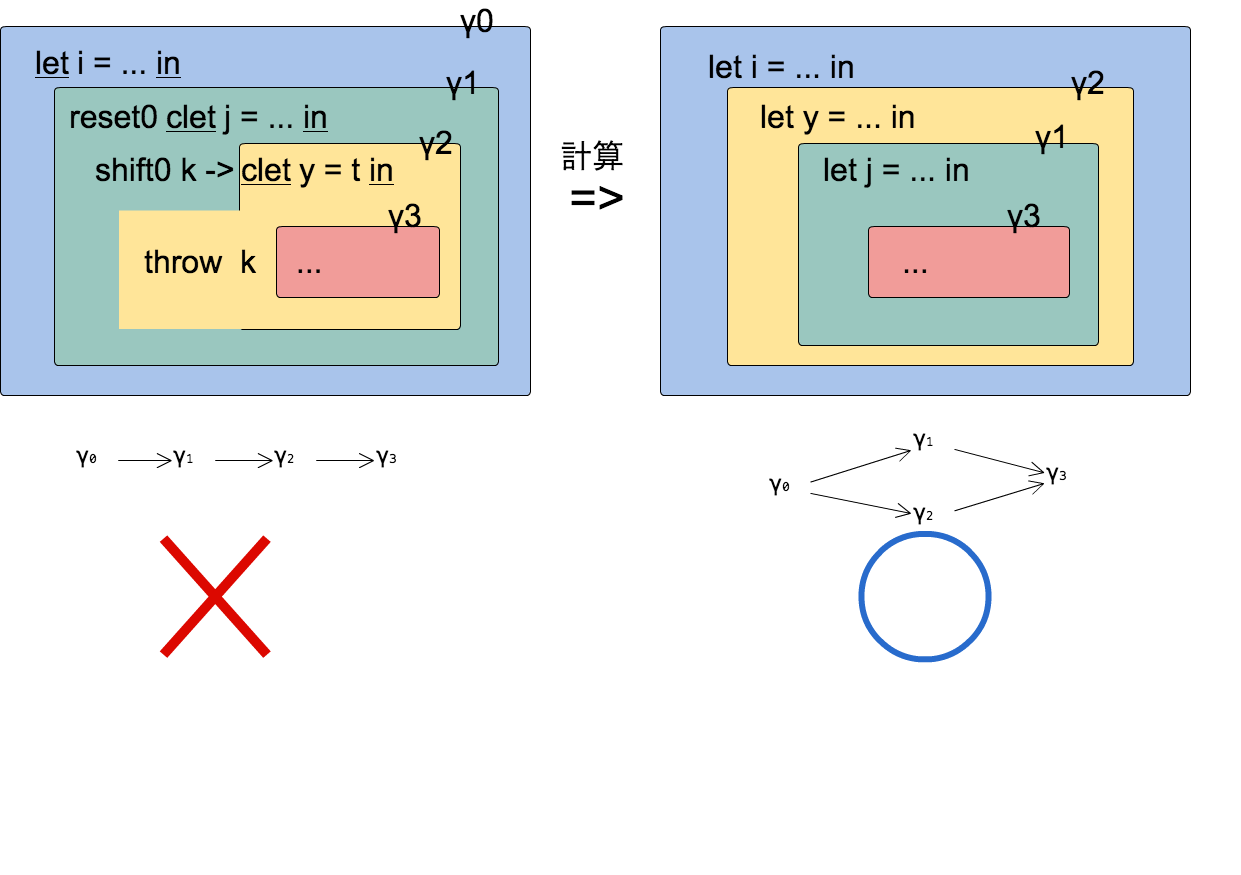
\includegraphics[clip,height=5.5cm]{./img/ecex_let.png}
\end{center}

しかし,shift0/reset0 が導入されることにより,計算の順序が

\begin{center}
  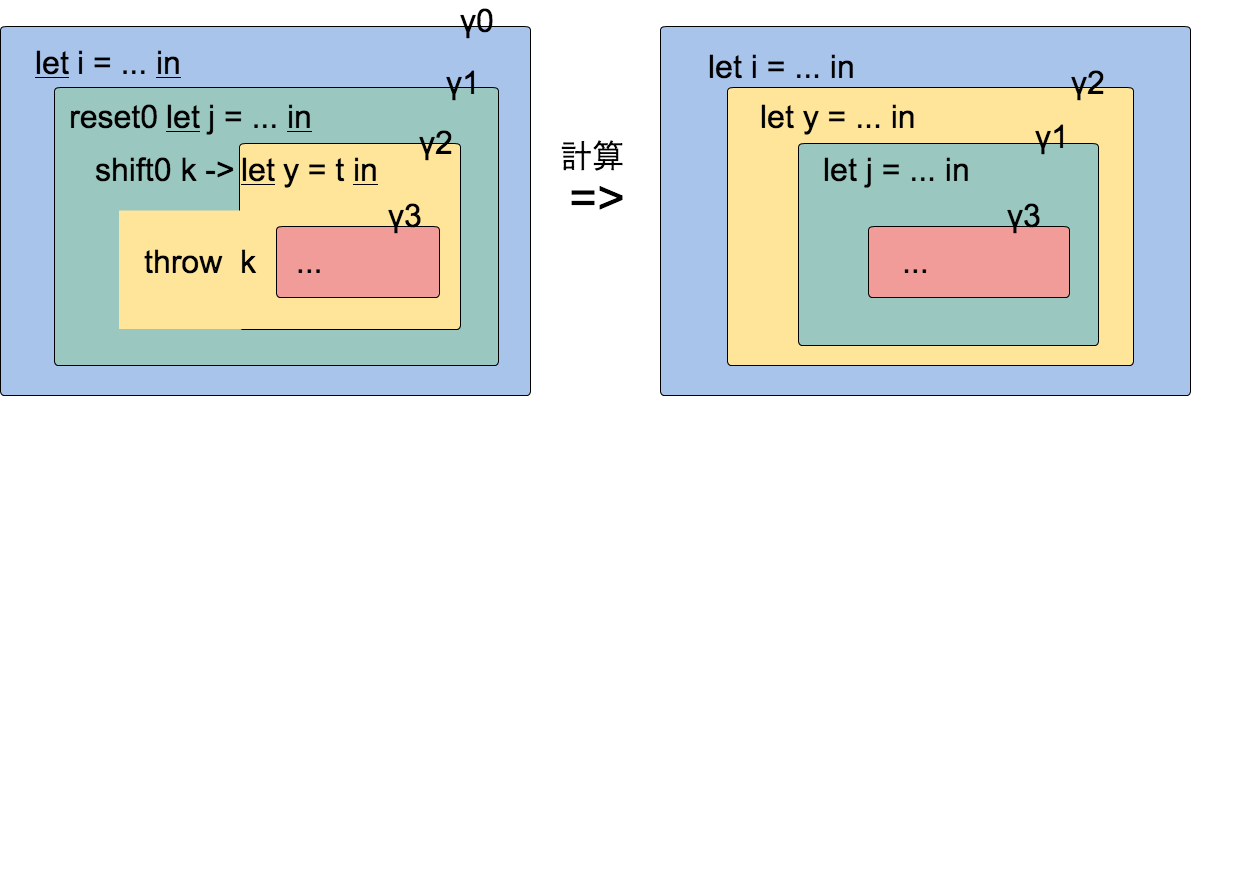
\includegraphics[clip,height=5.5cm]{./img/ecex_let_non_gamma.png}
\end{center}

\begin{center}
  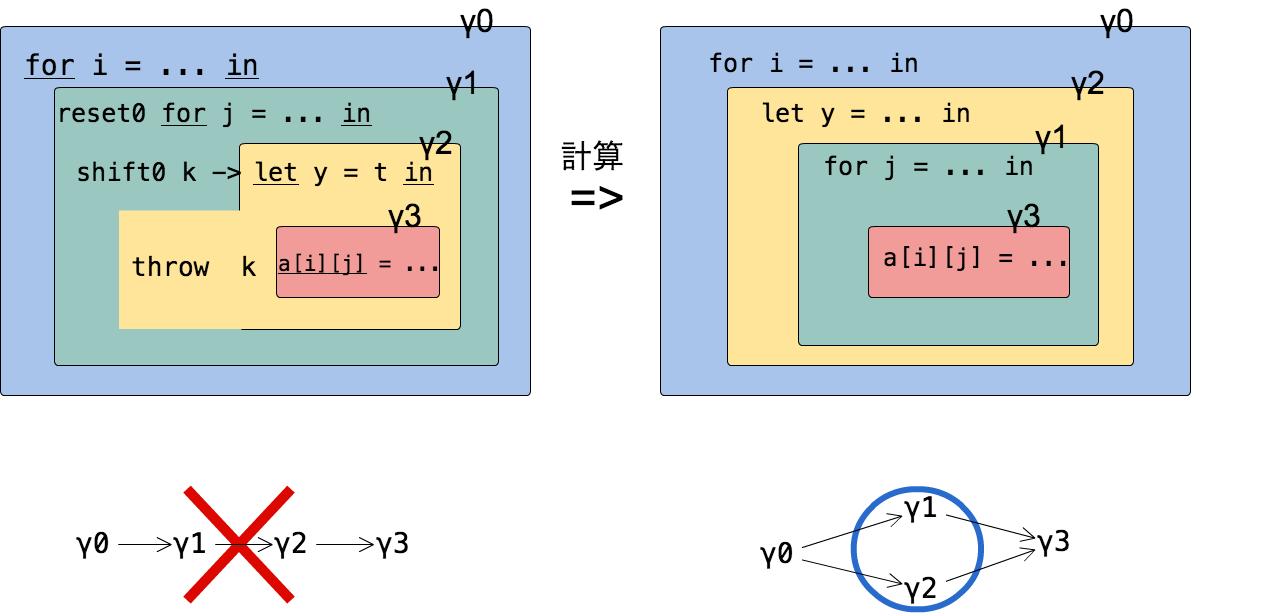
\includegraphics[clip,height=4cm]{./img/ecex_for.png}
\end{center}

\begin{center}
  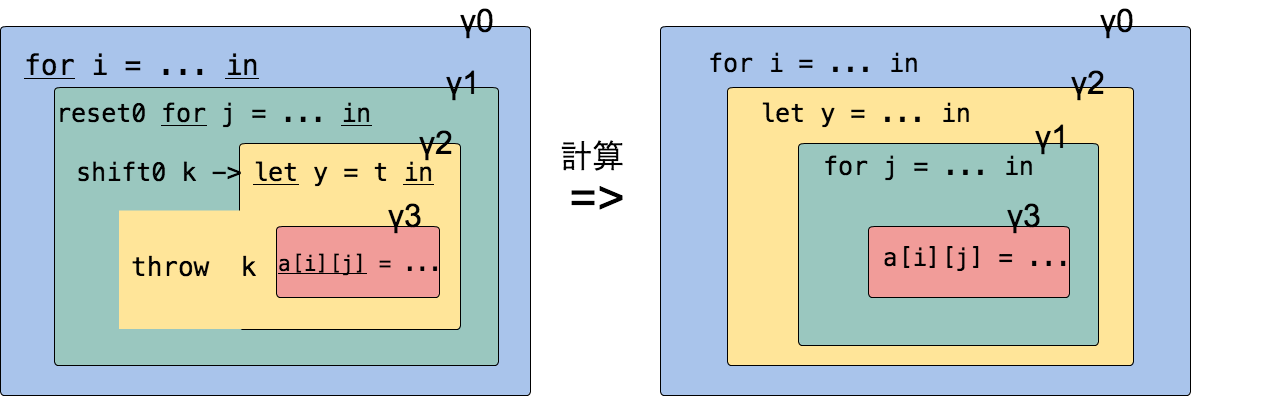
\includegraphics[clip,height=3cm]{./img/ecex_for_non_gamma.png}
\end{center}

\begin{center}
  
\includegraphics[clip,width=7cm]{./img/gamma.png}
\end{center}

\begin{center}
  
\includegraphics[clip,width=4cm]{./img/gamma_normal.png}
\end{center}

%%% Local Variables:
%%% mode: japanese-latex
%%% TeX-master: "paper"
%%% End:
